\documentclass{article}
\usepackage{graphicx} % Required for inserting images
\usepackage{pdfpages}
\usepackage{fancyhdr}
\usepackage{calc}
\usepackage{titlepic}
\usepackage{times}
\usepackage{mathptmx}
\usepackage[varg]{txfonts}
\usepackage{float}
\usepackage{pgfplots}
\usepackage{pgf-pie}
\usepackage{tcolorbox}
\usepackage[top=1cm,bottom=2cm,left=2cm,right=1.5cm]{geometry}

\title{Assignment 1} 
\author{ALI HASSAN ABDULHAKIM }
\date{7th October 2024}

\begin{document}

\begin{titlepage}
    \newcommand{\HRule}{\rule{\linewidth}{0.35mm}} % the horizontal lines, change thickness here
    \begin{flushleft}
        {\scriptsize
        \textbf{\large{China}}\\
        \vspace*{\stretch{0.010}}
        \textbf{\large{Northwestern Polytechnicl Univerity}}\\
        \vspace*{\stretch{0.010}}
        \textbf{\large{School of softwre }}\\
        \vspace*{\stretch{0.010}}

        \textbf{\large{Software Engineering}}}
    \end{flushleft}
    \HRule \\[0.3cm]
    \vspace*{\stretch{0.005}}
    \begin{center}
        \textbf{\textbf{\huge{Chapter One}}}\\
        \vspace*{\stretch{0.025}}
        Descriptive Statistics\\
        \vspace*{\stretch{0.015}}
        \textbf{\textsc{\large{Assignment }}}\\
    \end{center}
    \vspace*{\stretch{0.035}}
    \begin{center}
        prepared by\\
        \vspace*{\stretch{0.01}}
        \textbf{{\large ALI HASSAN ABDULHAKIM}}\\
        \vspace*{\stretch{0.01}}
        \textsc{{\large 2024280032}}\\
        \vspace*{\stretch{0.01}}
    \end{center}
    \begin{center}
        \vspace*{\stretch{0.035}}
        \textbf{\textsc{\huge{ Modern Maths and  Statistics}}}\\
        \vspace*{\stretch{0.02}}

        \HRule \\
        \vspace*{\stretch{0.015}}
    \end{center}

    \begin{center}
        \begin{tabular}{lll}
            \textbf{Professor:}  & \textsc{Xie Wenxian} 
            \tabularnewline
            \tabularnewline
        \end{tabular}
    \end{center}
    \sloppy
\end{titlepage}

\newpage

\section{{\huge 1.4.3 :}}

\begingroup

The data in Table 1.9 are presented to illustrate the role of renewable energy consumption in the U.S. energy supply
in 2007 (source: http://www.eia.doe.gov/fuelrenewable.html). Renewable energy consists of biomass, geothermal
energy, hydroelectric energy, solar energy, and wind energy.

\smallskip
\smallskip 
\textsc{(A)} Construct a bar graph \\
\textsc{(B)} Construct a Pareto chart.\\
\textsc{(C)} Construct a pie chart.

\endgroup

\newpage

\section*{Answer}

\begin{center}
    \textbf{\textbf{\huge{Answer}}}\\ 
\end{center}

\begingroup

The data in Table 1.9 are presented to illustrate the role of renewable energy consumption in the U.S. energy supply
in 2007 (source: http://www.eia.doe.gov/fuelrenewable.html). Renewable energy consists of biomass, geothermal
energy, hydroelectric energy, solar energy, and wind energy.

\smallskip
\smallskip 
\textsc{(A)} Construct a bar graph \\
\textsc{(B)} Construct a Pareto chart.\\
\textsc{(C)} Construct a pie chart.

\endgroup

\newpage

\section*{Answer}

\begin{center}
    \textbf{\textbf{\huge{Answer}}}\\ 
\end{center}

\begin{center}
    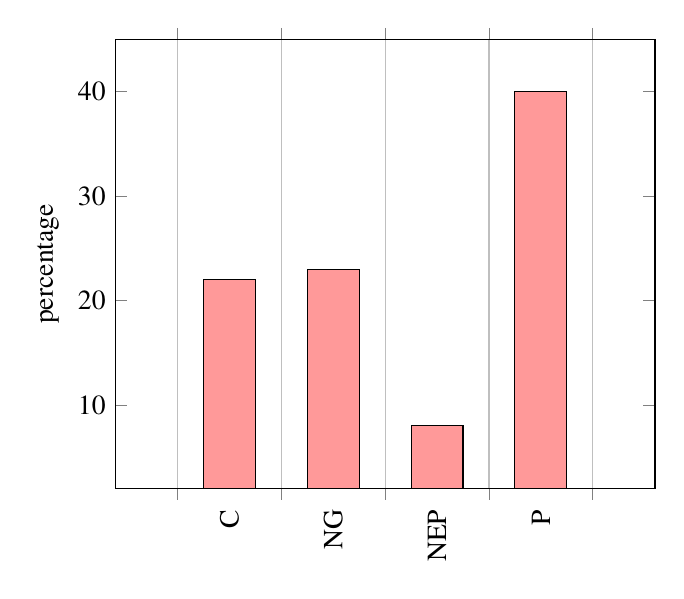
\begin{tikzpicture}
        \begin{axis}[every axis plot post,
            symbolic x coords={C,NG,NEP,P,RE},
            xtick=data, x tick label style = {rotate=90}, ylabel= percentage, ybar interval=.5, enlargelimits=0.15]
            \addplot [fill = red!40] coordinates{(C,22)(NG, 23)(NEP,8)(P, 40)(RE, 7)};   
        \end{axis}
    \end{tikzpicture}
\end{center}

\begin{center}
    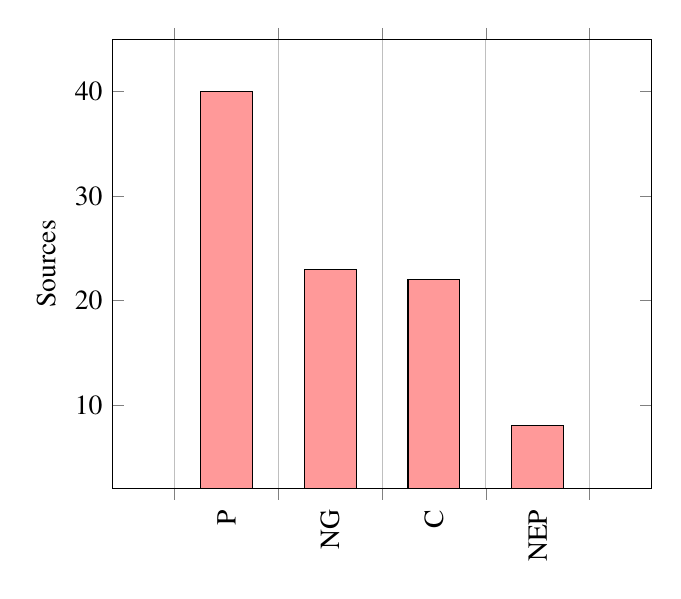
\begin{tikzpicture}
        \begin{axis}[every axis plot post,
            symbolic x coords={P, NG, C, NEP, RE},
            xtick=data, x tick label style = {rotate=90}, ylabel= Sources, ybar interval=.5, enlargelimits=0.15]
            \addplot [fill = red!40] coordinates{(P, 40)(NG, 23)(C,22)(NEP,8)(RE, 7)};   
        \end{axis}
    \end{tikzpicture}
\end{center}

% Add some space before the pie chart to make sure it's not right after the bar charts
\vspace{1cm}

\begin{center}
    % Pie chart
    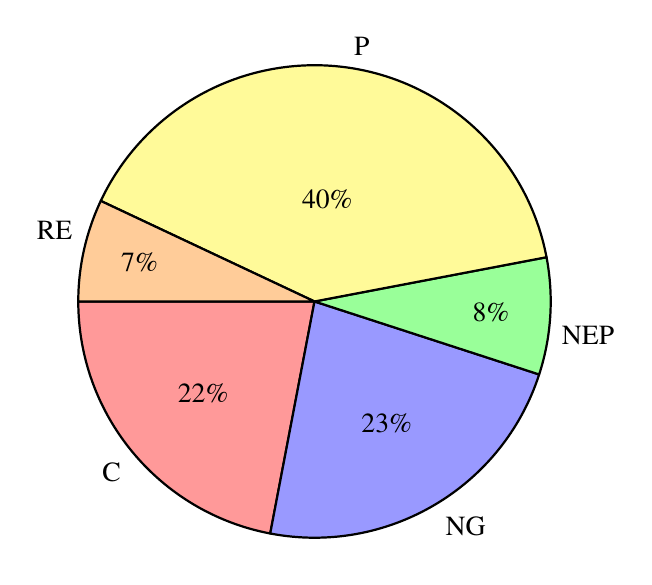
\begin{tikzpicture}
        \pie[rotate = 180, color = {red!40, blue!40, green!40, yellow!40, orange!40}]
        {22/C, 23/NG, 8/NEP, 40/P, 7/RE}
    \end{tikzpicture}
\end{center}


\newpage

\section{{\huge 1.4.14:}}

The following table gives radon concentrations in pCi/liter (picocurie per liter) obtained from 40 houses in a
certain area.

\begin{center}
    \begin{tabular}{c|c|c|c|c|c|c|c|c|c}
        2.9 & 0.6 & 13.5 & 17.1 & 2.8 & 3.8 & 16.0 & 2.1 & 6.4 & 17.2 \\
        7.9 & 0.5 & 13.7 & 11.5 & 2.9 & 3.6 & 6.1 & 8.8 & 2.2 & 9.4 \\
        15.9 & 8.8 & 9.8 & 11.5 & 12.3 & 3.7 & 8.9 & 13.0 & 7.9 & 11.7 \\
        6.2 & 6.9 & 12.8 & 13.7 & 2.7 & 3.5 & 8.3 & 15.9 & 5.1 & 6.0 \\ 
    \end{tabular} 
\end{center}

\smallskip
\smallskip 

\textsc{(A)} Construct a stem-and-leaf display and interpret.\\
\textsc{(B)} Construct a frequency histogram and interpret.\\
\textsc{(C)} Construct a pie chart and interpret.

\newpage

\section*{Answer}

\textbf{Stem and Leaf Plot}\\

\begin{center}
    \begin{tabular}{|c|l|}
        \hline
        \textbf{Stem} & \textbf{Leaves} \\
        \hline
        0 & 5 6 \\
        \hline
        1 & 5 5 7 9 \\
        \hline
        2 & 1 2 7 8 8 9 9 \\
        \hline
        3 & 5 6 7 8 \\
        \hline
        5 & 1 \\
        \hline
        6 & 0 1 2 4 9 \\
        \hline
        7 & 9 9 \\
        \hline
        8 & 3 8 8 9 \\
        \hline
        9 & 4 8 \\
        \hline
        11 & 5 5 7 \\
        \hline
        12 & 3 8 \\
        \hline
        13 & 0 5 7 7 \\
        \hline
        15 & 9 9 \\
        \hline
        16 & 0 \\
        \hline
        17 & 1 2 \\
        \hline
    \end{tabular}

 

    \begin{figure}[H]
        \centering
        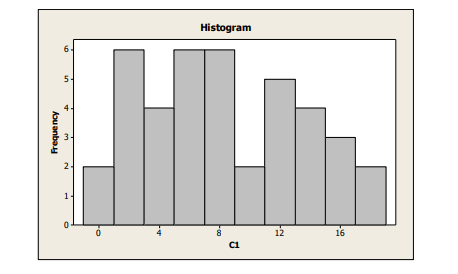
\includegraphics[width=0.5\textwidth]{histogram.png} % Adjust the width to your liking
        \caption{This is the histogram}
        \label{fig:image_label}
    \end{figure}
    \begin{figure}[H]
        \centering
        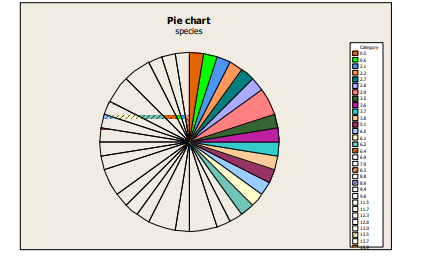
\includegraphics[width=0.5\textwidth]{pie.png} % Adjust the width to your liking
        \caption{Pie chart}
        \label{fig:image_label}
    \end{figure}
\end{center}

\end{document}
